\documentclass[uplatex,dvipdfmx]{jsarticle}
\usepackage{listings,jvlisting}
\usepackage{color}
\usepackage{xr}

\lstset{
  backgroundcolor=\color[rgb]{0.9,0.9,0.9},
  frame=single,
  basicstyle=\ttfamily
}
\makeatletter
\newcommand*{\addFileDependency}[1]{% argument=file name and extension
  \typeout{(#1)}
  \@addtofilelist{#1}
  \IfFileExists{#1}{}{\typeout{No file #1.}}
}
\makeatother

\newcommand*{\myexternaldocument}[1]{%
    \externaldocument{#1}%
    \addFileDependency{#1.tex}%
    \addFileDependency{#1.aux}%
}
\myexternaldocument{../categoryTheoryIntro/CategoryTheoryIntro}

\newcommand{\pr}[1]{\colorbox[rgb]{0.9,0.9,0.9}{\lstinline{#1}}}
\newcommand{\functype}[2]{\pr{#1 -> #2}}
\newcommand{\refcti}[1]{[CTI]\ref{#1}}
\newcommand{\fpmor}[3]{\pr{#1 :: #2 -> #3}}
\input{../categoryTheoryIntro/preemble.tex}
\begin{document}
\title{コエンドと余米田の補題}
\maketitle
  \begin{define}[モノイダル圏]
    ある圏$\cat{C}$がモノイダル圏であるとは、
    \begin{quote}
      \begin{mydescription}
        \item[モノイド積関手]
        ある関手$\functor{\otimes}{C\times C}{C}$が存在する。またこの積で表される対象をテンソル積と呼ぶ。
        \item[単位対象]圏$\cat{C}$のある対象$I$が存在する。またこの対象を単位対象と呼ぶ。
        \item[結合子]ある射$\mor{a_{ABC}}{(A\otimes B)\otimes C}{A\otimes(B\otimes C)}$が存在して同型射となる。また$A,B,C$に対して自然。
        \item[左単位子]ある射$\mor{I\otimes C}{C}$が存在して同型射となる。また$C$に対して自然。
        \item[右単位子]ある射$\mor{C\otimes I}{C}$が存在して同型射となる。また$C$に対して自然。
        \item[三角恒等式]以下の等式を満たす必要がある。
        \[(id_X\otimes l_Y)\circ a_{XIY}=r_X\otimes id_Y\]
        \item[五角恒等式]以下の等式を満たす必要がある。
        \[a_{WXY\otimes Z}\circ a_{W\otimes XYZ}=(id_W\otimes a)\circ a_{WX\otimes YZ}\circ(a_{WXY}\otimes id_Z) \]
      \end{mydescription}
    \end{quote}
  \end{define}
  三角恒等式と五角恒等式についての説明は省略するが、これを示すと$\otimes$の射関数の適用、$a,l,r$とその逆射や恒等射で構成される自然変換の図式が自然に可換になる。
  \begin{prop}
    $\cat{H}$はモノイダル圏である。
  \end{prop}
  \begin{proof}
    \begin{quote}~
      \begin{mydescription}
        \item[モノイド積関手]
        モノイド積関手を双積関手$\functor{(-\times -)}{H\times H}{H}$とする。
        \item[単位対象]単位対象を終対象$1$とする。
        \item[結合子]対象$(A\times B)\times C$が$A$と$B\times C$における積であることを示せば良い。
        射影射$\mor{\pi_A\circ\pi_{A\times B}}{(A\times B)\times C}{A}$、$\mor{\pi_B\times id_C}{(A\times B)\times C}{B\times C}$とし、任意の射$\mor{f}{X}{A}$と射$\mor{g}{X}{B\times C}$に対する射の対を$\tuple{\tuple{f,\pi_B\circ g},\pi_C\circ g}$とする。
        \begin{center}
          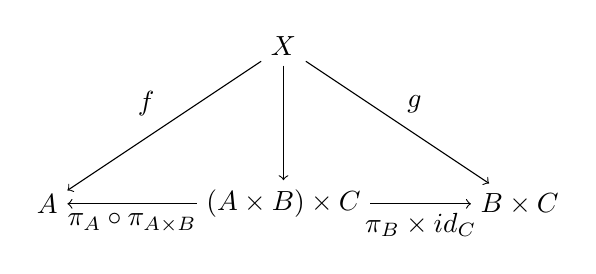
\begin{tikzpicture}[auto]
            \node (X) at (0, 0) {$X$};
            \node (AB_C) at (0, -2) {$(A\times B)\times C$};
            \node (A) at (-3, -2) {$A$};
            \node (BC) at (3, -2) {$B\times C$};

            \draw[->] (X) to node[swap]{$f$}(A);
            \draw[->] (X) to node{$g$}(BC);
            \draw[->] (X) to node{}(AB_C);
            \draw[->] (AB_C) to node{$\pi_A\circ\pi_{A\times B}$}(A);
            \draw[->] (AB_C) to node[swap]{$\pi_B\times id_C$}(BC);
          \end{tikzpicture}
        \end{center}
        この時、
        \begin{align*}
          \pi_A\circ\pi_{A\times B}\circ\tuple{\tuple{f,\pi_B\circ g},\pi_C\circ g}&=\pi_A\circ\tuple{f,\pi\circ g}\\
          &=f\\
          (\pi_B\times id_C)\circ\tuple{\tuple{f,\pi_B\circ g},\pi_C\circ g}&=\tuple{\pi_B\circ g,\pi_C\circ g}\\
          &=g
        \end{align*}
        であるから$\tuple{\tuple{f,\pi_B\circ g},\pi_C\circ g}$は確かに射の対である。
        一意性については
        \begin{align*}
          (\pi_A\circ\pi_{A\times B})\circ h &= f\\
          (\pi_B\times id_C)\circ h &= g
        \end{align*}
        を満たすような任意の射$\mor{h}{X}{(A\times B)\times C}$に対して$h=\tuple{\tuple{f,\pi_B\circ g},\pi_C\circ g}$を示せば良い。

        ここで$h$は$(A\times B)\times C$における射の対であるから、\[h=\tuple{\pi_{A\times B}\circ h,\pi_C\circ h}\]である。これによって
        \begin{align*}
          (\pi_B\times id_C)\circ h &= (\pi_B\times id_C) \tuple{\pi_{A\times B}\circ h,\pi_C\circ h}\\
          &=\tuple{\pi_B\circ\pi_{A\times B}\circ h,\pi_C\circ h}\\
          \pi_B\circ g &= \pi_B\circ\pi_{A\times B}\circ h\\
          \pi_C\circ g &= \pi_C\circ h
        \end{align*}
        が成り立つ。

        また、$\pi_{A\times B}\circ h$もまた$A\times B$の射の対であるから、\[\pi_{A\times B}\circ h=\tuple{\pi_A\circ\pi_{A\times B}\circ h,\pi_B\circ\pi_{A\times B}\circ h}\]である。よって\[h = \tuple{\tuple{\pi_A\circ\pi_{A\times B}\circ h,\pi_B\circ\pi_{A\times B}\circ h},\pi_C\circ h}\]が成り立つ。
        ここから$h$を消すように代入すると、\[h = \tuple{\tuple{f,\pi_B\circ g},\pi_C\circ g}\]となり、一意性が示せた。
        
        ここで積同士の同型による同型射はお互いの射影射の対であったから、結合子\[\mor{a_{ABC}}{(A\times B)\times C}{A\times (B\times C)}\]は
        \[a_{ABC}=\tuple{\pi_A\circ\pi_{A\times B},\pi_B\times id_C}\]となる。

        あとは自然性を示せばよいが、かなり複雑になるため省略する。
        \item[左単位子]
        命題\refcti{prop-product-with-terminal-object}と\refcti{prop-naturality-of-a-and-a1}を参照
        \item[右単位子]
        命題\refcti{prop-product-with-terminal-object}と\refcti{prop-naturality-of-a-and-a1}を参照
        \item[三角恒等式]省略
        \item[五角恒等式]省略
      \end{mydescription}
    \end{quote}
  \end{proof}

  \begin{define}[対称モノイダル圏]
    圏$\cat{C}$が対称モノイダル圏であるとは、$\cat{C}$がモノイダル圏であり、$\mor{c_{AB}}{A\times B}{B\times A}$が$\mor{c_{BA}}{B\times A}{A\times B}$を逆射とする自然同型であり、以下の等式を満たす時である。
    \[a_{YZX}\circ c_{X,Y\otimes Z}\circ a_{XYZ}=(id_Y\otimes c_{XZ})\circ a_{YXZ}\circ(c_{XY}\otimes id_Z)\]
    \[r_{X}\circ c_{IX} = l_{X}\]
  \end{define}
  \begin{prop}
    圏$\cat{H}$は対称モノイダル圏である。
  \end{prop}
  \begin{prop}[自然変換の普遍性]\label{prop-university-of-nat}
    圏$\cat{C}$の任意の対象$C$に対して$\cat{Set}$の射$\mor{\lambda_C}{\arset{\funccat{C}{D}}{F}{G}}{\arset{D}{FC}{GC}}$が存在し、$\cat{C}$の任意の射$\mor{f}{A}{B}$に対して、\[\arset{D}{FA}{Gf}\circ\lambda_A=\arset{D}{Ff}{GB}\circ\lambda_B\]を満たす。
    
    \begin{center}
      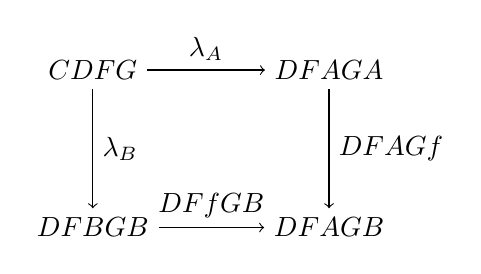
\begin{tikzpicture}[auto]
        \node (FG) at (0, 0) {$\arset{\funccat{C}{D}}{F}{G}$};
        \node (FAGA) at (3, 0) {$\arset{D}{FA}{GA}$};
        \node (FBGB) at (0, -2) {$\arset{D}{FB}{GB}$};
        \node (FAGB) at (3, -2) {$\arset{D}{FA}{GB}$};

        \draw[->] (FG) to node{$\lambda_A$}(FAGA);
        \draw[->] (FG) to node{$\lambda_B$}(FBGB);
        \draw[->] (FAGA) to node{$\arset{D}{FA}{Gf}$}(FAGB);
        \draw[->] (FBGB) to node{$\arset{D}{Ff}{GB}$}(FAGB);

      \end{tikzpicture}
    \end{center}
    
    またある対象$X$に対しても任意の対象$C$に対する$\mor{\mu_C}{\arset{\funccat{C}{D}}{F}{G}}{\arset{D}{FC}{GC}}$が存在し、\[\arset{D}{FA}{Gf}\circ\mu_A=\arset{D}{Ff}{GB}\circ\mu_B\]を満たすのであれば、
    \begin{center}
      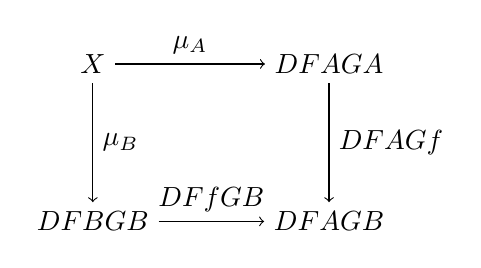
\begin{tikzpicture}[auto]
        \node (FG) at (0, 0) {$X$};
        \node (FAGA) at (3, 0) {$\arset{D}{FA}{GA}$};
        \node (FBGB) at (0, -2) {$\arset{D}{FB}{GB}$};
        \node (FAGB) at (3, -2) {$\arset{D}{FA}{GB}$};

        \draw[->] (FG) to node{$\mu_A$}(FAGA);
        \draw[->] (FG) to node{$\mu_B$}(FBGB);
        \draw[->] (FAGA) to node{$\arset{D}{FA}{Gf}$}(FAGB);
        \draw[->] (FBGB) to node{$\arset{D}{Ff}{GB}$}(FAGB);

      \end{tikzpicture}
    \end{center}
    任意の対象$C$に対して$\mu_C=\lambda_C\circ h$を満たすような射$\mor{h}{X}{\arset{\funccat{C}{D}}{F}{G}}$が一意に存在する。すなわち、$\mu_C=\lambda_C\circ h'$を満たすような$h'$が存在すれば、$h'=h$が成り立つ。
    \begin{center}
      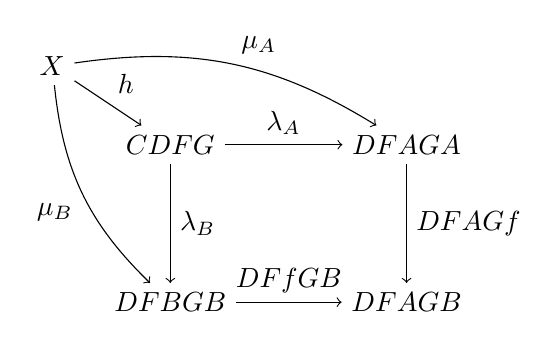
\begin{tikzpicture}[auto]
        \node (FG) at (0, 0) {$\arset{\funccat{C}{D}}{F}{G}$};
        \node (X) at (-1.5, 1) {$X$};
        \node (FAGA) at (3, 0) {$\arset{D}{FA}{GA}$};
        \node (FBGB) at (0, -2) {$\arset{D}{FB}{GB}$};
        \node (FAGB) at (3, -2) {$\arset{D}{FA}{GB}$};

        \draw[->] (FG) to node{$\lambda_A$}(FAGA);
        \draw[->] (X) to node{$h$}(FG);

        \draw[->] (FG) to node{$\lambda_B$}(FBGB);
        \draw[->,bend left = 20] (X) to node{$\mu_A$}(FAGA);
        \draw[->,bend right = 20] (X) to node[swap]{$\mu_B$}(FBGB);
        \draw[->] (FAGA) to node{$\arset{D}{FA}{Gf}$}(FAGB);
        \draw[->] (FBGB) to node{$\arset{D}{Ff}{GB}$}(FAGB);

      \end{tikzpicture}
    \end{center}
  \end{prop}
  \begin{proof}
    まず任意の対象$C$に対する$\cat{Set}$の射$\mor{\lambda_C}{\arset{\funccat{C}{D}}{F}{G}}{\arset{D}{FC}{GC}}$を定義する。\\
    任意の自然変換$\nat{\alpha}{F}{G}$に対して$\lambda_C(\alpha)=\alpha_C$とする。任意の自然変換はある対象に対する成分をただ一つ持つから、この操作は写像であり、$\cat{Set}$の射である。すると、
    \begin{align*}
      \arset{D}{FA}{Gf}\circ\lambda_A(\alpha)&=\arset{D}{FA}{Gf}(\alpha_A)&\text{($\lambda$の定義)}\\
      &=Gf\circ\alpha_A&\text{(射写像の定義)}\\
      \arset{D}{Ff}{GB}\circ\lambda_B(\alpha)&=\arset{D}{Ff}{GB}(\alpha_B)&\text{($\lambda$の定義)}\\
      &=\alpha_B\circ Ff&\text{(射写像の定義)}
    \end{align*}
  であり、$\alpha$の自然性から$Gf\circ\alpha_A=\alpha_B\circ Ff$が成り立つ。よって$\arset{D}{FA}{Gf}\circ\lambda_A=\arset{D}{Ff}{GB}\circ\lambda_B$を満たす。\\
  この等式では自然変換の成分が写像で与えられた場合の自然性を射写像を用いて課していることが分かる。\\
  次に射$h$の存在と一意性を示そうと思う。そこでまずは任意の対象$X$に終対象$1$を当てはめて考える。射$\mor{\mu_C}{1}{\arset{D}{FC}{GC}}$は射$\mor{\mu_A}{FA}{GA}$であり、任意の対象$C$に対して存在する。更に仮定より$\arset{D}{FA}{Gf}\circ\mu_A=\arset{D}{Ff}{GB}\circ\mu_B$が成り立つ。
  \begin{align*}
    \arset{D}{FA}{Gf}\circ\mu_A&=\arset{D}{Ff}{GB}\circ\mu_B\\
    \arset{D}{FA}{Gf}(\mu_A)&=\arset{D}{Ff}{GB}(\mu_B)&\text{(元と終対象からの射の同一視)}\\
    Gf\circ\mu_A&=\mu_B\circ Ff&\text{(射写像の定義)}
  \end{align*}
  よって自然変換の定義より、$\mu_C$は対象$C$成分であることが分かる。この自然変換を$\nat{\mu}{F}{G}$とすると、$\mu$は$\arset{\funccat{C}{D}}{F}{G}$の元である。すなわち$\mor{\mu}{1}{\arset{\funccat{C}{D}}{F}{G}}$と表せる。ここで$h=\mu$とすると$\lambda$は成分を取る写像であったから、$\mu_C=\lambda_C(\mu)=\lambda_C\circ\mu=\lambda_C\circ h$が成り立つ。
  \begin{center}
    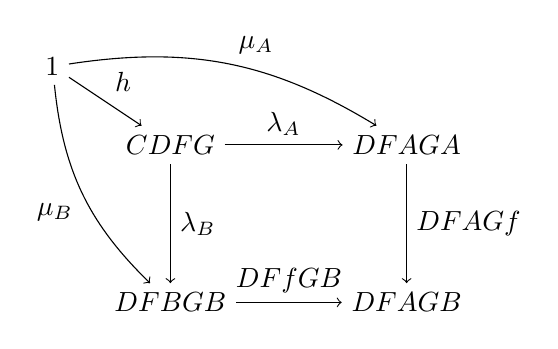
\begin{tikzpicture}[auto]
      \node (FG) at (0, 0) {$\arset{\funccat{C}{D}}{F}{G}$};
      \node (X) at (-1.5, 1) {$1$};
      \node (FAGA) at (3, 0) {$\arset{D}{FA}{GA}$};
      \node (FBGB) at (0, -2) {$\arset{D}{FB}{GB}$};
      \node (FAGB) at (3, -2) {$\arset{D}{FA}{GB}$};

      \draw[->] (FG) to node{$\lambda_A$}(FAGA);
      \draw[->] (X) to node{$h$}(FG);

      \draw[->] (FG) to node{$\lambda_B$}(FBGB);
      \draw[->,bend left = 20] (X) to node{$\mu_A$}(FAGA);
      \draw[->,bend right = 20] (X) to node[swap]{$\mu_B$}(FBGB);
      \draw[->] (FAGA) to node{$\arset{D}{FA}{Gf}$}(FAGB);
      \draw[->] (FBGB) to node{$\arset{D}{Ff}{GB}$}(FAGB);
    \end{tikzpicture}
  \end{center}
  一意性に関しても、$\mu_C=\lambda_C\circ h'$であるような$h'$が存在したとしても、$\mu_C={h'}_C$であり、自然変換の定義から$h'=\mu=h$が成り立つ。\\
  次に対象$1$を任意の対象$X$に拡張しよう。$X$の任意の元$x$に対し$\mu_C(x)$はある自然変換の$C$成分である。上記の議論から自然変換$h(x)_C=\mu_C(x)$であるため、自然変換$h(x)$は任意の$x$に対して一意に存在することになる。よって条件を満たす$h$は存在する。
  一意性に関しても、$\mor{h'}{\arset{\funccat{C}{D}}{F}{G}}{\arset{D}{FA}{GA}}$が存在して\[\lambda_C\circ h' = \mu_C\]が成り立ったとしても、任意の元$x$に対して\[\lambda_C\circ h'(x) = \mu_C(x)\]が成り立つから、$h'(x)=h(x)$となる。よって$h = h'$であり、一意性が示せた。

  \begin{center}
    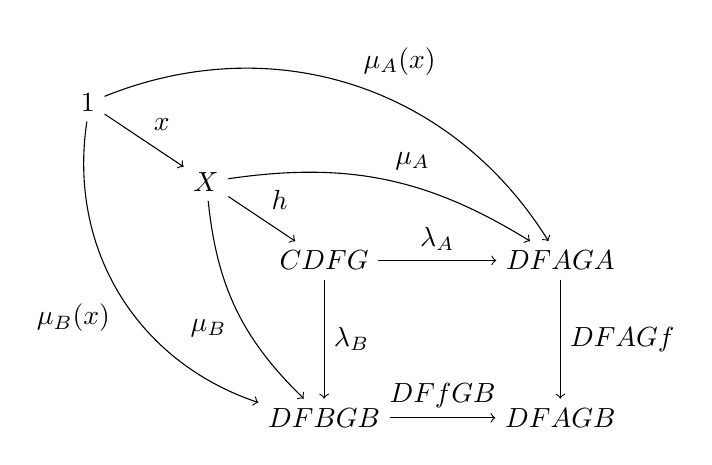
\begin{tikzpicture}[auto]
      \node (FG) at (0, 0) {$\arset{\funccat{C}{D}}{F}{G}$};
      \node (X) at (-1.5, 1) {$X$};
      \node (1) at (-3, 2) {$1$};
      \node (FAGA) at (3, 0) {$\arset{D}{FA}{GA}$};
      \node (FBGB) at (0, -2) {$\arset{D}{FB}{GB}$};
      \node (FAGB) at (3, -2) {$\arset{D}{FA}{GB}$};
      \draw[->] (FG) to node{$\lambda_A$}(FAGA);
      \draw[->] (X) to node{$h$}(FG);
      \draw[->] (1) to node{$x$}(X);
      \draw[->] (FG) to node{$\lambda_B$}(FBGB);
      \draw[->,bend left = 20] (X) to node{$\mu_A$}(FAGA);
      \draw[->,bend right = 20] (X) to node[swap]{$\mu_B$}(FBGB);
      \draw[->,bend left = 40] (1) to node{$\mu_A(x)$}(FAGA);
      \draw[->,bend right = 40] (1) to node[swap]{$\mu_B(x)$}(FBGB);
      \draw[->] (FAGA) to node{$\arset{D}{FA}{Gf}$}(FAGB);
      \draw[->] (FBGB) to node{$\arset{D}{Ff}{GB}$}(FAGB);
    \end{tikzpicture}
    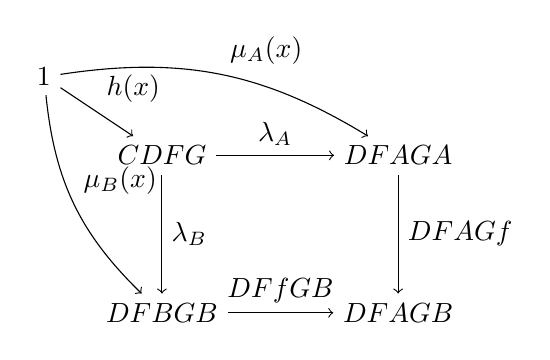
\begin{tikzpicture}[auto]
      \node (FG) at (0, 0) {$\arset{\funccat{C}{D}}{F}{G}$};
      \node (X) at (-1.5, 1) {$1$};
      \node (FAGA) at (3, 0) {$\arset{D}{FA}{GA}$};
      \node (FBGB) at (0, -2) {$\arset{D}{FB}{GB}$};
      \node (FAGB) at (3, -2) {$\arset{D}{FA}{GB}$};
      \draw[->] (FG) to node{$\lambda_A$}(FAGA);
      \draw[->] (X) to node{$h(x)$}(FG);
      \draw[->] (FG) to node{$\lambda_B$}(FBGB);
      \draw[->,bend left = 20] (X) to node{$\mu_A(x)$}(FAGA);
      \draw[->,bend right = 20] (X) to node{$\mu_B(x)$}(FBGB);
      \draw[->] (FAGA) to node{$\arset{D}{FA}{Gf}$}(FAGB);
      \draw[->] (FBGB) to node{$\arset{D}{Ff}{GB}$}(FAGB);
    \end{tikzpicture}
  \end{center}
\end{proof}
\begin{define}[エンド]\label{def-end}
  ある圏$\cat{C,D}$と、関手$\functor{F}{C^{op}\times C}{D}$に対するエンド$(\displaystyle\int_{c:\cat{C}} F(C,C),\lambda)$を以下のように構成する。
  \begin{quote}
    \begin{mydescription}
      \item[エンド対象]圏$\cat{D}$のある対象$\displaystyle\int_{c:\cat{C}} F(C,C)$
      \item[射影射] 圏$\cat{C}$の任意の対象$X$に対して$\mor{\lambda_C}{\displaystyle\int_{c:\cat{C}} F(C,C)}{F(X,X)}$なる射が存在し、圏$\cat{C}$の任意の射$\mor{f}{A}{B}$に対して$F(A,f)\circ\lambda_A=F(f,B)\circ\lambda_B$が成り立つ。
      \begin{center}
        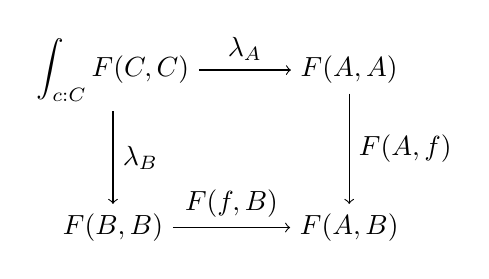
\begin{tikzpicture}[auto]
          \node (FG) at (0, 0) {$\displaystyle\int_{c:\cat{C}} F(C,C)$};
          \node (FAGA) at (3, 0) {$F(A,A)$};
          \node (FBGB) at (0, -2) {$F(B,B)$};
          \node (FAGB) at (3, -2) {$F(A,B)$};
  
          \draw[->] (FG) to node{$\lambda_A$}(FAGA);  
          \draw[->] (FG) to node{$\lambda_B$}(FBGB);
          \draw[->] (FAGA) to node{$F(A,f)$}(FAGB);
          \draw[->] (FBGB) to node{$F(f,B)$}(FAGB);
        \end{tikzpicture}
      \end{center}
      \item[普遍性] $F$に対して同様の条件を満たす$(Y,\mu)$が存在する時、任意の対象$X$において$\mu=\lambda_X\circ h$が成り立つような$\mor{h}{Y}{\displaystyle\int_{c:\cat{C}} F(C,C)}$が一意に存在する。
      \begin{center}
        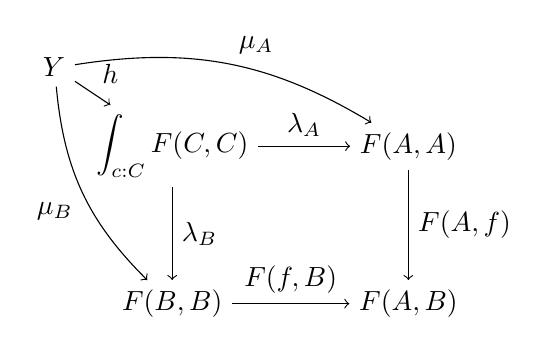
\begin{tikzpicture}[auto]
          \node (FG) at (0, 0) {$\displaystyle\int_{c:\cat{C}} F(C,C)$};
          \node (X) at (-1.5, 1) {$Y$};
          \node (FAGA) at (3, 0) {$F(A,A)$};
          \node (FBGB) at (0, -2) {$F(B,B)$};
          \node (FAGB) at (3, -2) {$F(A,B)$};
  
          \draw[->] (FG) to node{$\lambda_A$}(FAGA);
          \draw[->] (X) to node{$h$}(FG);
  
          \draw[->] (FG) to node{$\lambda_B$}(FBGB);
          \draw[->,bend left = 20] (X) to node{$\mu_A$}(FAGA);
          \draw[->,bend right = 20] (X) to node[swap]{$\mu_B$}(FBGB);
          \draw[->] (FAGA) to node{$F(A,f)$}(FAGB);
          \draw[->] (FBGB) to node{$F(f,B)$}(FAGB);
        \end{tikzpicture}
      \end{center}
    \end{mydescription}
  \end{quote}
\end{define}
\begin{prop}
  エンド対象を取る操作は関手$\functor{\scriptsize\int_{c:\cat{C}}}{\funccat{C^{op}\times C}{D}}{D}$である。
\end{prop}
\begin{proof}
  極限の場合と同様に構成、証明できる。
\end{proof}
\begin{define}[コエンド]\label{def-coend}
  ある圏$\cat{C,D}$と、関手$\functor{F}{C^{op}\times C}{D}$に対するコエンド$(\displaystyle\int^{c:\cat{C}} F(C,C),\kappa)$を以下のように構成する。
  \begin{quote}
    \begin{mydescription}
      \item[コエンド対象]圏$\cat{D}$のある対象$\displaystyle\int^{c:\cat{C}} F(C,C)$
      \item[入射] 圏$\cat{C}$の任意の対象$X$に対して$\mor{\kappa_C}{\displaystyle\int^{c:\cat{C}} F(C,C)}{F(X,X)}$なる射が存在し、圏$\cat{C}$の任意の射$\mor{f}{B}{A}$に対して$\kappa_A\circ F(A,f)=\kappa_B\circ F(f,B)$が成り立つ。
      \begin{center}
        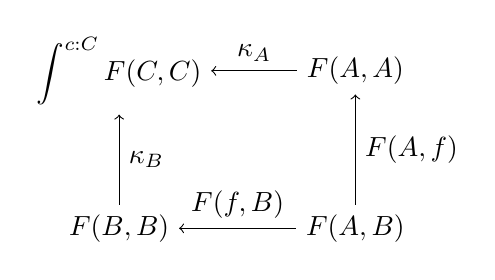
\begin{tikzpicture}[auto]
          \node (FG) at (0, 0) {$\displaystyle\int^{c:\cat{C}} F(C,C)$};
          \node (FAGA) at (3, 0) {$F(A,A)$};
          \node (FBGB) at (0, -2) {$F(B,B)$};
          \node (FAGB) at (3, -2) {$F(A,B)$};
  
          \draw[<-] (FG) to node{$\kappa_A$}(FAGA);  
          \draw[<-] (FG) to node{$\kappa_B$}(FBGB);
          \draw[<-] (FAGA) to node{$F(A,f)$}(FAGB);
          \draw[<-] (FBGB) to node{$F(f,B)$}(FAGB);
        \end{tikzpicture}
      \end{center}
      \item[普遍性] $F$に対して同様の条件を満たす$(Y,\mu)$が存在する時、任意の対象$X$において$\mu=h\circ \kappa_X$が成り立つような$\mor{h}{\displaystyle\int^{c:\cat{C}} F(C,C)}{Y}$が一意に存在する。
      \begin{center}
        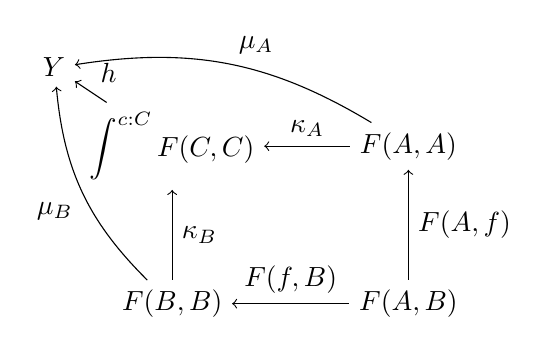
\begin{tikzpicture}[auto]
          \node (FG) at (0, 0) {$\displaystyle\int^{c:\cat{C}} F(C,C)$};
          \node (X) at (-1.5, 1) {$Y$};
          \node (FAGA) at (3, 0) {$F(A,A)$};
          \node (FBGB) at (0, -2) {$F(B,B)$};
          \node (FAGB) at (3, -2) {$F(A,B)$};
  
          \draw[<-] (FG) to node{$\kappa_A$}(FAGA);
          \draw[<-] (X) to node{$h$}(FG);
  
          \draw[<-] (FG) to node{$\kappa_B$}(FBGB);
          \draw[<-,bend left = 20] (X) to node{$\mu_A$}(FAGA);
          \draw[<-,bend right = 20] (X) to node[swap]{$\mu_B$}(FBGB);
          \draw[<-] (FAGA) to node{$F(A,f)$}(FAGB);
          \draw[<-] (FBGB) to node{$F(f,B)$}(FAGB);
        \end{tikzpicture}
      \end{center}
    \end{mydescription}
  \end{quote}
\end{define}
\begin{prop}[米田の補題]
  任意の圏$\cat{C}$の対象$A$と関手$\functor{F}{C}{Set}$において
  \[FA\cong\arset{\funccat{C}{Set}}{\arset{C}{A}{-}}{F}\]であり、$A,F$に対して自然。
\end{prop}
\begin{proof}[同型性]
同型射をラムダ表記を用いて
\[\phi(a) = \lambda f.Ffa\]
\[\phi^{-1}(\alpha) = \alpha_A(id_A)\]とする。また$\phi(a)$が自然変換であることは簡単に示せる。
\[(Ff\circ\phi(a)_B)(g) = f(g(a)) = f\circ g(a) = (\phi(a)_C\circ\arset{C}{A}{f})(g)\]
\begin{center}
  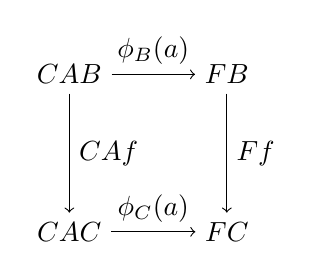
\begin{tikzpicture}[auto]
    \node (ab) at (0, 0) {$\arset{C}{A}{B}$};
    \node (ac) at (0, -2) {$\arset{C}{A}{C}$};
    \node (fb) at (2, 0) {$FB$};
    \node (fc) at (2, -2) {$FC$};
    \draw[->] (ab) to node{$\arset{C}{A}{f}$}(ac);
    \draw[->] (fb) to node{$Ff$}(fc);  
    \draw[->] (ab) to node{$\phi_B(a)$}(fb);
    \draw[->] (ac) to node{$\phi_C(a)$}(fc);  
  \end{tikzpicture}
\end{center}
$A$の任意の元$a$に対して
\begin{align*}
  \phi^{-1}\circ\phi(a) &= (\lambda f.Ffa)_A(id_A)\\
  &=F(id_A)(a)\\
  &=a
\end{align*}
であるから$\phi^{-1}\circ\phi=id_A$である。
また任意の自然変換$\alpha$に対して
\begin{align*}
  \phi\circ\phi^{-1}(\alpha) &= \lambda f.Ff(\alpha_A(id_A))\\
  &=\lambda f.(Ff\circ\alpha_A)(id_A)\\
  &=\lambda f.(\alpha_{\cod(f)}\circ\arset{C}{A}{f})(id_A)&\text{($\alpha$の自然性)}\\
  &=\lambda f.\alpha_{\cod(f)}(f)
\end{align*}
$\phi(a)$の自然性より$\lambda f.\alpha_{\cod(f)}(f)$はこのような形の自然変換\[\nat{\lambda f.\alpha_{\cod(f)}(f)}{\arset{C}{A}{-}}{F}\]である。

任意の射$\mor{g}{A}{B}$に対して
\[(\lambda f.\alpha_{\cod(f)}(f))_B(g)=\alpha_B(g)\]であるから\[(\lambda f.\alpha_{\cod(f)}(f))_B=\alpha_B\]であり、\[\lambda f.\alpha_{\cod(f)}(f)=\alpha\]となる。よって$\phi\circ\phi^{-1}(\alpha)=\alpha$であり、$\phi\circ\phi^{-1}=ID$
\end{proof}
この証明において重要な部分は$\phi\circ\phi^{-1}=ID$における$\alpha_A(id_A)$から$\alpha$への復元である。とくに$\alpha$の自然性によって$\alpha$の成分$\mor{\alpha_B}{\arset{C}{A}{B}}{FB}$が定義できる任意の対象$B$に対してそれが導出できる。さらに$\arset{C}{A}{f}(id_A)=f$によってそのような成分$\alpha_B$の元の対応関係が具体的に示されるのである。

\begin{proof}[自然性]
  対象$A$と関手$F$における同型射を$\phi_{AF},\ \phi^{-1}_{AF}$とし、$A$に対する自然性を示す。すなわち任意の射$\mor{f}{A}{B}$に対して、\[Ff\circ\phi^{-1}_{AF}=\phi^{-1}_{BF}\circ\arset{\funccat{C}{Set}}{\arset{C}{f}{-}}{F}\]を示せば良い。
  \begin{center}
    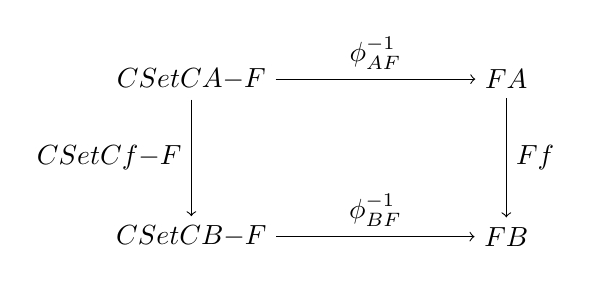
\begin{tikzpicture}[auto]
      \node (ab) at (0, 0) {$\arset{\funccat{C}{Set}}{\arset{C}{A}{-}}{F}$};
      \node (ac) at (0, -2) {$\arset{\funccat{C}{Set}}{\arset{C}{B}{-}}{F}$};
      \node (fb) at (4, 0) {$FA$};
      \node (fc) at (4, -2) {$FB$};
      \draw[->] (ab) to node[swap]{$\arset{\funccat{C}{Set}}{\arset{C}{f}{-}}{F}$}(ac);
      \draw[->] (fb) to node{$Ff$}(fc);
      \draw[->] (ab) to node{$\phi^{-1}_{AF}$}(fb);
      \draw[->] (ac) to node{$\phi^{-1}_{BF}$}(fc);  
    \end{tikzpicture}
  \end{center}
  また紛らわしいが、二つの反変関手の合成で得られるため$\arset{\funccat{C}{Set}}{\arset{C}{A}{-}}{F}$は$A$に対して共変である。
  任意の自然変換$\nat{\alpha}{\arset{C}{A}{-}}{F}$に対して
  \begin{align*}
    Ff\circ\phi^{-1}_{AF}(\alpha) &= Ff\circ\alpha_A(id_A)\\
    \phi^{-1}_{BF}\circ\arset{\funccat{C}{Set}}{\arset{C}{f}{-}}{F}(\alpha) &= (\alpha_B\circ\arset{C}{f}{B})(id_B)\\
    &=\alpha_B(f)\\
    &=(\alpha_B\circ\arset{C}{A}{f})(id_A)\\
  \end{align*}
  $\alpha$の自然性より$Ff\circ\alpha_A=\alpha_B\circ\arset{C}{A}{f}$であるから、$(\alpha_B\circ\arset{C}{A}{f})(id_A)=Ff\circ\alpha_A(id_A)$であり、$A$に対して自然であることが示せた。次に$F$に対して自然であることを示す。つまり任意の自然変換$\nat{\beta}{F}{G}$に対して
  \[\alpha_A\circ\phi^{-1}_{AF} = \phi^{-1}_{AG}\circ\arset{\funccat{C}{Set}}{\arset{C}{A}{-}}{\beta}\]を示せば良い。
  \begin{center}
    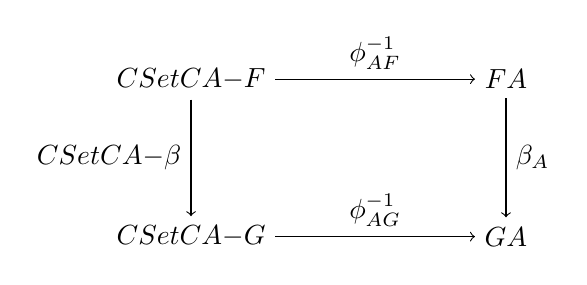
\begin{tikzpicture}[auto]
      \node (ab) at (0, 0) {$\arset{\funccat{C}{Set}}{\arset{C}{A}{-}}{F}$};
      \node (ac) at (0, -2) {$\arset{\funccat{C}{Set}}{\arset{C}{A}{-}}{G}$};
      \node (fb) at (4, 0) {$FA$};
      \node (fc) at (4, -2) {$GA$};
      \draw[->] (ab) to node[swap]{$\arset{\funccat{C}{Set}}{\arset{C}{A}{-}}{\beta}$}(ac);
      \draw[->] (fb) to node{$\beta_A$}(fc);
      \draw[->] (ab) to node{$\phi^{-1}_{AF}$}(fb);
      \draw[->] (ac) to node{$\phi^{-1}_{AG}$}(fc);  
    \end{tikzpicture}
  \end{center}
  任意の自然変換$\nat{\alpha}{\arset{C}{A}{-}}{F}$に対して、
  \begin{align*}
    \alpha_A\circ\phi^{-1}_{AF}(\alpha) &= \beta_A(\alpha_A(id_A))\\
    &=\beta_A\circ\alpha_A(id_A)
    \phi^{-1}_{AG}\circ\arset{\funccat{C}{Set}}{\arset{C}{A}{-}}{\beta} &= (\beta\cdot\alpha)_A(id_A)\\
  \end{align*}
  自然変換の垂直合成より$\beta_A\circ\alpha_A=(\beta\cdot\alpha)_A$であるから、$\alpha_A\circ\phi^{-1}_{AF}(\alpha)=\phi^{-1}_{AG}\circ\arset{\funccat{C}{Set}}{\arset{C}{A}{-}}{\beta}$であり、$F$に対しても自然であることが分かる。
\end{proof}
自然変換の集合はエンドで表せるから、米田の補題は\[FA\cong\displaystyle\int_{c:\cat{C}} \arset{Set}{\arset{C}{A}{C}}{FC}\]とも表せる。
\begin{define}[反変米田の補題]
  任意の圏$\cat{C}$の対象$A$と関手$\functor{F}{C^{op}}{Set}$において
  \[FA\cong\arset{\funccat{C^{op}}{Set}}{\arset{C}{-}{A}}{F}\]であり、$A,F$に対して自然。
\end{define}
\begin{define}[余米田の補題]
  任意の圏$\cat{C}$と対象$A$と関手$\functor{F}{C}{Set}$において
  \[FA\cong\displaystyle\int^{c:\cat{C}}FC\times\arset{C}{C}{A}\]
  またここでの積分記号はエンドではなくコエンドである。
\end{define}
\begin{proof}
  証明略。米田の補題などを用いて同型の計算で証明できる。
\end{proof}
また、$\displaystyle\int^{c:\cat{C}}FC\times\arset{C}{C}{A}$の性質を考えると、以下の性質が成り立つ。
任意の射$\mor{f}{B}{C}$において$FB$の任意の元$b$と任意の射$\mor{g}{C}{A}$の組$\tuple{b,g}$に対し\[\kappa_B(b,g\circ f)=\kappa_A(Ff(c),g)\]が成り立つ。また同様の性質が$(X,\mu)$でも成り立つ、つまり\[\mu_B(b,g\circ f)=\mu_A(Ff(b),g)\]である時、一意な射$\mor{h}{\displaystyle\int^{c:\cat{C}}FC\times\arset{C}{C}{A}}{X}$が存在し、$\mu$は$\kappa$によって$h$へ分解される。すなわち$\mu_A = h\circ\kappa_A$である。
\begin{center}
  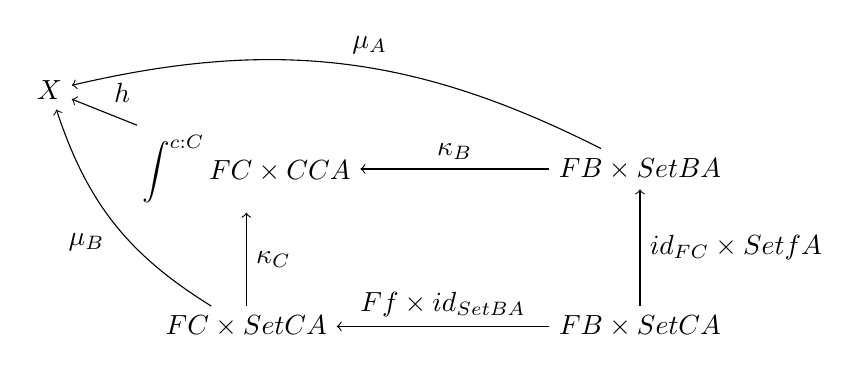
\begin{tikzpicture}[auto]
    \node (FG) at (0, 0) {$\displaystyle\int^{c:\cat{C}}FC\times\arset{C}{C}{A}$};
    \node (X) at (-2.5, 1) {$X$};
    \node (FAGA) at (5, 0) {$FB\times\arset{Set}{B}{A}$};
    \node (FBGB) at (0, -2) {$FC\times\arset{Set}{C}{A}$};
    \node (FAGB) at (5, -2) {$FB\times\arset{Set}{C}{A}$};

    \draw[<-] (FG) to node{$\kappa_B$}(FAGA);
    \draw[<-] (X) to node{$h$}(FG);

    \draw[<-] (FG) to node{$\kappa_C$}(FBGB);
    \draw[<-,bend left = 20] (X) to node{$\mu_A$}(FAGA);
    \draw[<-,bend right = 20] (X) to node[swap]{$\mu_B$}(FBGB);
    \draw[<-] (FAGA) to node{$id_{FC}\times \arset{Set}{f}{A}$}(FAGB);
    \draw[<-] (FBGB) to node{$Ff\times id_{\arset{Set}{B}{A}}$}(FAGB);
  \end{tikzpicture}
\end{center}
余米田の補題で述べていることは、$\displaystyle\int^{c:\cat{C}}FC\times\arset{C}{C}{A}$を$FA$へ置き換えてもこのような普遍性が成り立つということである。
\end{document}

https://hackage.haskell.org/package/optics-0.4.2/docs/Optics.html
coend calculus
https://arxiv.org/pdf/1501.02503.pdf